\documentclass[12pt,a4paper]{article}
\usepackage[utf8]{inputenc}
\usepackage[czech]{babel}
\usepackage[T1]{fontenc}
\usepackage{amsmath}
\usepackage{amsfonts}
\usepackage{amssymb}
\usepackage{color,graphicx}
\usepackage{epstopdf}
\usepackage{indentfirst}
\setlength{\parindent}{4em} 
\author{Jakub Drápela}
\usepackage{fancyhdr}
\usepackage{siunitx}
\usepackage{pdflscape}
\usepackage[backend=bibtex,style=numeric,backref=true]{biblatex}
\definecolor{black}{gray}{0}
\usepackage[pdftex,unicode]{hyperref}
\hypersetup{colorlinks,pdfhighlight=/O,citecolor=black,
  filecolor=black,urlcolor=black,linkcolor=black,
  breaklinks=true,pdfpagemode=UseNone,plainpages=false,
}
\usepackage{filecontents}  % create "citations.bib" on-the-fly
\graphicspath{{./imgs/}}

%\fontfamily{phs}
%\selectfont

\begin{filecontents*}{podnik_zamer.bib}

@online{pict,
 author  = "The New York Times",
 title   = "The Amazon Echo",
 year    = "2015",
 urlseen = "03-17-16",
 url     = "http://static01.nyt.com/images/2015/06/25/business/GADGETWISE/GADGETWISE-master675.jpg",
}
\end{filecontents*}
\addbibresource{podnik_zamer.bib}

\begin{document}
\pagestyle{empty}

%%nastaveni pisma  
%\fontfamily{phv}
%\selectfont

	\begin{center}

\large

České vysoké učení technické v Praze\\
\medskip
Fakulta elektrotechnická\\[2cm]
{\LARGE\bfseries Household Intelligent Assistant}

\vfill
\begin{figure}[h!]
\begin{center}

\includegraphics[width = 5cm]{logo.pdf} 
\end{center}
\end{figure}
\vfill

\begin{tabular}{rl}

Autoři: & Jiří Burant \\
\noalign{\vspace{1mm}}
		& Jakub Drápela \\
		\noalign{\vspace{1mm}}
		& Martin Klučka\\
		\noalign{\vspace{1mm}}
		& Petr Kovář \\
		\noalign{\vspace{1mm}}
		& Jakub Konrád\\
		\noalign{\vspace{1mm}}
		& Pavel Trutman\\
\noalign{\vspace{2mm}}
Studijní obor: & Kybernetika a robotika \\
\noalign{\vspace{2mm}}
Datum vypracování: & \today\\
\end{tabular}

\end{center}

\newpage
\pagestyle{plain}     % zapne obyčejné číslování
\setcounter{page}{1}
%% zahlaví a zápatí
\addtolength{\voffset}{-3cm}
\addtolength{\headheight}{2cm}

\pagestyle{fancy}
\lhead{
\includegraphics[scale=0.12]{cvut_text.jpg}  }
\rhead{\textbf{Household Intelligent Assistant}}
%\rhead{\textit{\bfseries Burant,Drápela,Klučka,Kovář,Konrád,Trutman}}
\lfoot{}
\cfoot{\thepage}
\rfoot{}
\renewcommand{\headrulewidth}{0.4pt}


\section*{Popis projektu, motivace}
Jako lidé si stále klademe různé otázky. Abychom mohli ve světě rozumně fungovat potřebujeme na tyto otázky znát odpovědi. Od té doby, co se začaly informace zaznamenávat lze odpovědi nalézt v záznamech. V nedávné historii lidé prahnoucí po informacích ve velkém kupovali knihy, noviny, jízdní řády, prostě média se žádaným obsahem. 

My se snažíme udělat krok vpřed. Ruční hledání informací obejít a nechat si informaci vyhledat automaticky nástrojem, který můžeme ovládat jednoduše hlasem.

V České republice je přibližně 10 milionů obyvatel. Určitě si dokážete představit, že mnoho z nich by systém ovládaný hlasem uvítalo. V první řadě se jedná o hendikepované osoby, kterým by tento systém velmi ulehčil život. Užitečný je ale i pro uživatele, kteří mají inteligentní domáctnost nebo používají zabezpečovací zařízení. Právě tento systém jim umožní všechny tyto inteligentní části domácnosti propojit v jeden funční celek a tím si usnadnit ovládání celého domova. Tak jak roste trh \textit{Internet of Things}, se bude poptávka po těchto systémech zvyšovat, až jednou budou v každé domáctnosti. Právě proto je tento trh perspektivní a je výhodné do něj investovat.

\section*{Detailní specifikace}
Zaměříme se na vytvoření dialogového systému pro použití v běžné domácnosti či kanceláři. Tedy systému, který bude čekat na vyřčení aktivačního slova a poté bude poslouchat příkaz uživatele. Následně vyhodnotí dotaz a sdělí příslušnou odpověď uživateli. Bude umět sám odpovídat na kladené otázky z limitované oblasti počasí, dopravy, obecných informací atd. K realizaci projektu použijeme již existující knihovny, které vhodně propojíme do funkčního celku.

V prvotní fázi se zaměříme pouze na otázky z oboru počasí, času a lokace. Systém tedy nebude mít takový rozsah jako jiné podobné aplikace, ale tento rozsah půjde v budoucnosti jednoduše rozšířit.

Výhoda tohoto projektu je, že bude vyvíjen jako otevřený software a bude vysoce modulární. Každý si tak bude moci tento systém sám rozšřit a upravit podle svých potřeb.

\section*{Současná řešení na trhu}
V současné době existuje řada aplikací, které fungují na podobném principu. Uveďme například aplikaci \textbf{Cortana} od firmy Microsoft. Cortana, podobně jako další aplikace \textbf{Siri} od firmy Apple, je označována jako osobní asistent. Lze ji použít pro širokou škálu úkonů. Například hlasové ovládání přijímače nebo vyhledávání informací na internetu. Její nevýhodou je použití pouze pod operačním systémem Windows, případně iOS. 

Jako další lze uvést open-source aplikaci \textbf{Jasper} v jazyce Python. Tato aplikace umožňuje využití hlasu pro získání informací. Můžeme ji také použít v inteligentním bydlení a v dalších situacích. Jelikož je volně dostupná, lze k ní libovolně přidávat nové moduly a její použití ještě rozšířit. Stává se tak pro nás vhodnou inspirací. 

Za zmínku ještě stojí projekt \textbf{Amazon Echo} od firmy Amazon. Tento osobní asistent umí přehrávat hudbu, odpovídat na otázky, vyhledávat zprávy, zjišťovat počasí, vytvářet seznamy a mnoho dalších věcí. 

\section*{Popis navrženého řešení}
Samotná finální aplikace se bude skládat z aplikačního jádra a modulů, které budou zodpovědné za jednotlivé funkcionality aplikace. Jádro aplikace bude pouze volat jednotlivé moduly a bude jim předávat získaná data z ostatních modulů. Bude tedy řídit celý běh aplikace, ale nebude v něm probíhat žádné zpracování informací. Naopak jednotlivé moduly budou úzce zaměřené na zpracování nebo zjištění konkrétních dat. Mezi jádrem aplikace a jednotlivými moduly bude striktně definované rozhraní, což nám snadno umožní jednotlivé moduly nahradit za jiné, aniž by bylo třeba upravit jádro aplikace nebo ostatní moduly. Protože je aplikace vyvíjena jako otevřený software, umožňuje tato vysoká modularita každému uživateli jednoduché vytvoření vlastního modulu, případně úpravu stávajích modulů. Blokové schéma aplikace je zobrazeno na obrázku \ref{fig:diagram api}.

\begin{figure}[ht]
	\begin{center}
	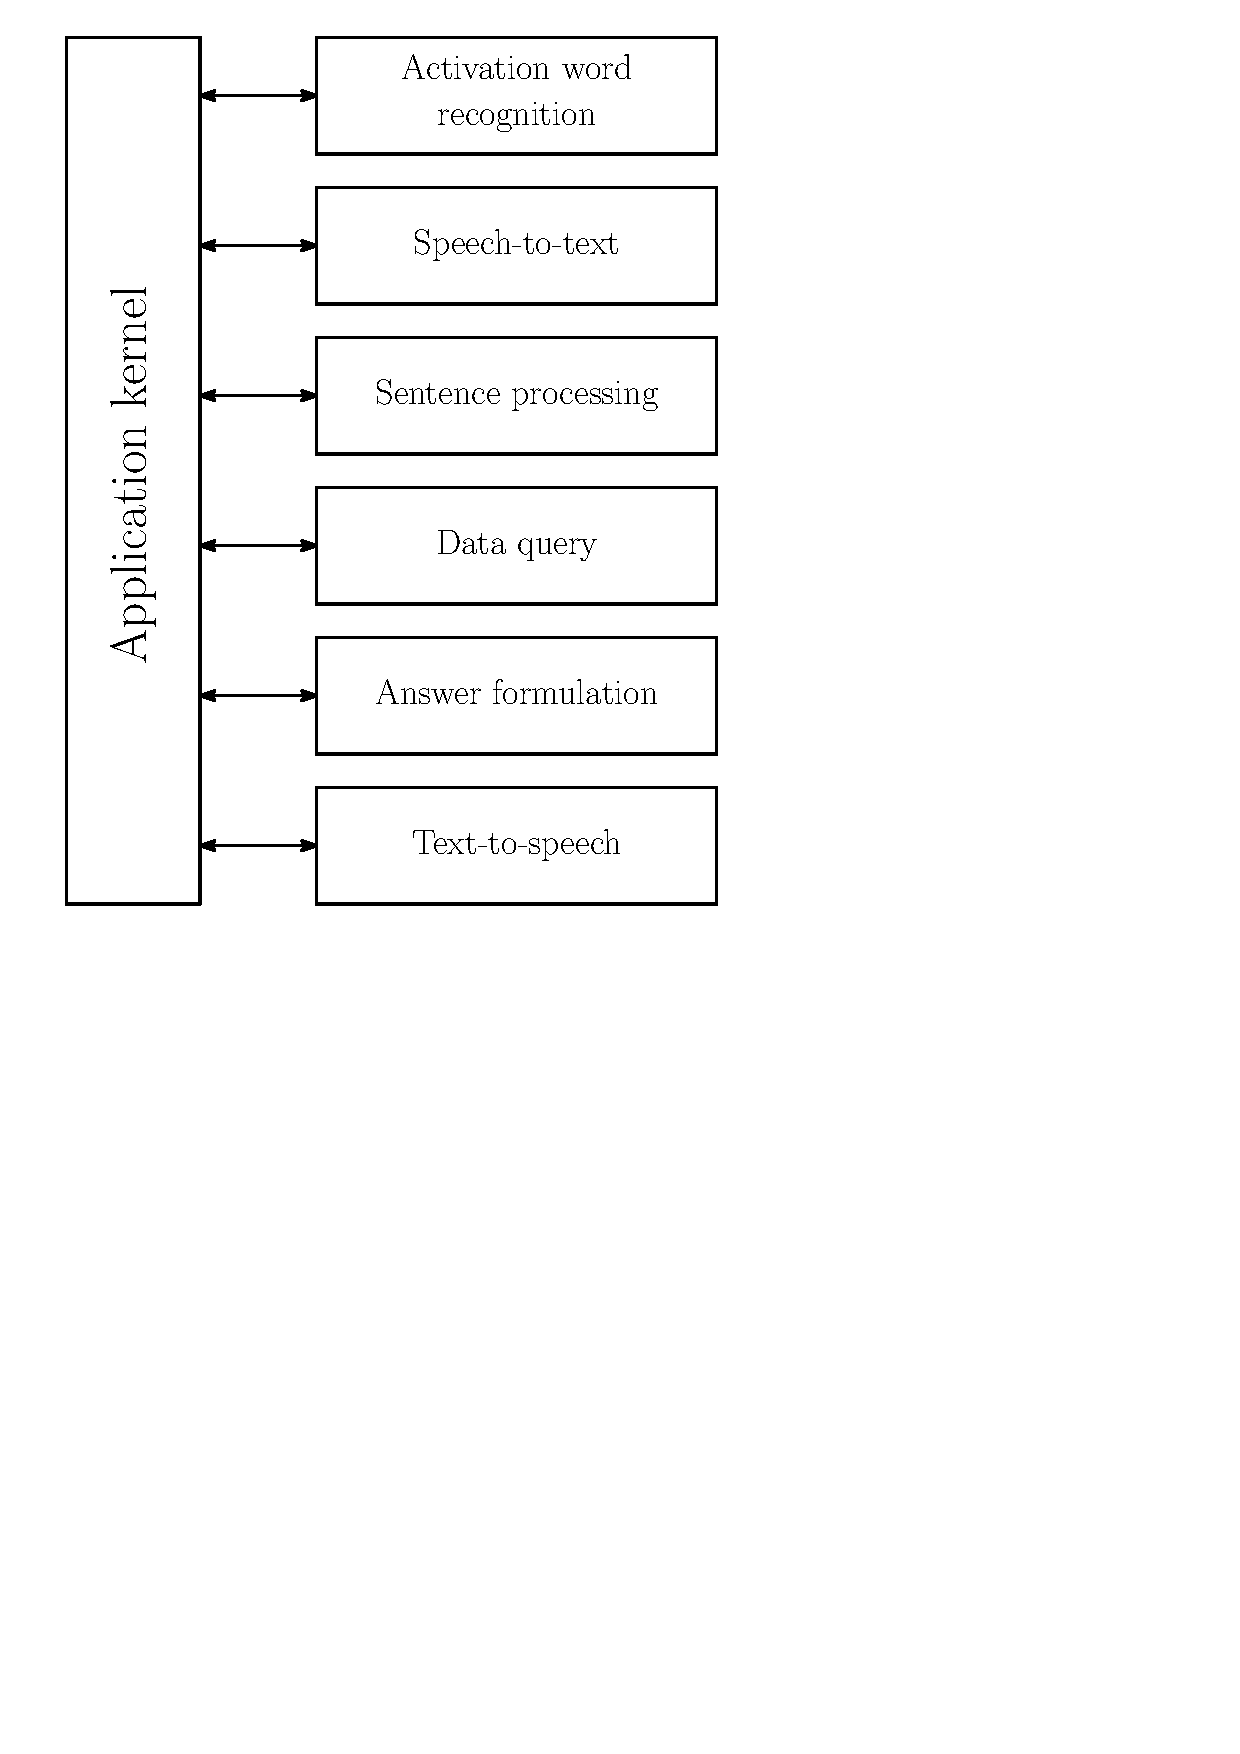
\includegraphics[height = 9cm]{blockDiagram.pdf}
	\caption{Blokový diagram navrženého řešení projektu Household Intelligent Assistant.}
	\label{fig:diagram api}
	\end{center}
\end{figure}

Při popisu návrhu řešení aplikace budeme postupovat tak, jak bude reakce na mluvené slovo postupně prostupovat mezi jednotlivými moduly, až nakonec vznikne finální odpověď ve formě mluveného slova.

Za běžného provozu bude aplikace ve stand-by režimu, ve kterém bude čekat na zaznění aktivačního slova. Na rozpoznání aktivačního slova bude vyhrazen jeden samostatný modul. Aktivační slovo by mělo být snadno rozlišitelné od ostatních a zvukově velmi výrazné, aby nedocházelo k jeho záměně s hlukem na pozadí. Ukazuje se vhodné zvolit tříslabičné slovo s výraznými hláskami a vokály jako například \uv{a} nebo \uv{x}.

Po zaznění aktivačního slova uživatelem se aktivuje blok pro rozpoznání mluveného slova, který převede položenou otázku na prostý text. Vhodnou robustní knihovnou pro tento problém je třeba vybrat. Jako vhodné knihovny se ukazují třeba \textit{wit.ai} nebo \textit{PocketSphinx}. Tyto knihovny podrobněji prozkoumáme a vybereme tu, která bude při řešení daného problému nejúspěšnější.

Ze textu, který jsme obdrželi v předchozím kroku, je třeba získat jeho význam. Toho docílíme buď pomocí indetifikátoru klíčových slov (již zmiňovaná knihovna \textit{PocketSphinx}) nebo podle porovnání dotazu s databází naší aplikace a odhadem jeho významu (\textit{wit.ai}).

Získaný význam dotazu je vstupní hodnotou do modulu, který vyhledá potřebné informace na internetu. Jednotlivé okruhy informací budou obstarávat jednotlivé subsystémy. Jeden subsystém bude například zpracovát pouze dotazy z oblasti počasí. Vhodnou aplikací pro tento okruh se jeví \textit{forecast.io}.

Informace získané z internetu je třeba přeformulovat do srozumitelné odpovědi podle předem zadaných vzorů. To bude úkolem dalšího samostatného modulu.

V poslední řadě využijeme aplikaci k převedení formulované odpovědi do strojově mluvené řeči. Prvotní aplikací pro tento převod bude jednoduchý \textit{"The Festival Speech Synthesis System"}. Později se pokusíme o využití jiné aplikace s propracovanějším převodem textu na řeč.

% plus dopsat nějaké kecy kolem 

\section*{Plán projektu}
Vytvořili jsme časový plán projektu, který obsahuje naplánovanou posloupnost jednotlivých činností s datem jejich plnění a klíčové milníky. Harmonogram projektu je graficky znázorněn formou Ganttova diagramu na obr. \ref{fig:diagram gantt}. Ganttův diagram zobrazuje ve sloupcích časová období a v řádcích jednotlivé plány.

Diagram obsahuje pět stěžejních fází projektu. První dvě fáze projektu, diskuze nad řešením projektu a rozdělení rolí v týmu, již proběhly. Následuje realizace prvotního prototypu s omezenými schopnostmi. Prototyp následně postoupí fázi rozšiřování o nové možnosti a v poslední řadě přichází na řadu testování a finální úprava. Harmonogram projektu zahrnuje, kromě časového rozložení jednotlivých úkolů a milníků, také pravidelné týdenní schůze, termíny odevzdání průběžných zpráv a prezentace stavu projektu.

\section*{Analýza rizik a krizové plány}
V průběhu řešení projektu mohou nastat situace, které budou bránit jeho plynulé a bezproblémové realizaci. Analyzovali jsme rizika, která mohou nastat a připravili jsme pro ně odpovídající krizové plány tak, aby bylo možné efektivní řešení vzniklých problémů a došlo k minimalizaci případných negativních následků. \\

\noindent \textbf{Rizika projektu}, která mohou nastat a \textbf{plány} na jejich eliminaci: 

\begin{itemize}
	\item{\textbf{Nedostatečná funkčnost některého z modulů}} - jednotlivé moduly, které využívají již existující knihovny nebudou mít dostatečnou funkčnost.
	
        Náš projekt se z velké části spoléhá na již existující knihovny. Těch je dostupné velké množství a rozsah jejich funkcionality se různí. Je tedy nutné zvolit vhodné knihovny tak, aby splňovaly požadavky našeho projektu a případně jejich funkce doplnit. Pokud se nám nepodaří vhodné knihovny nalézt, bude nutné je doprogramovat.

	\item{\textbf{Nemoc}} - v dlouhodobém řešení projektu zastihne některého člena týmu vážná nemoc. 
	
	V tomto případě zastoupí nemocného člena jiný člen a práce se přeorganizuje tak, aby nevznikaly zbytečné prodlevy. Obdobně budeme jednat, pokud někdo z týmu nebude stíhat plnit zadanou práci, a to z jakéhokoliv důvodu.
	
	\item{\textbf{Finance}} - nebude k dispozici dostatek financí.
	
	Budeme využívat volně dostupných programů. Nebude tak potřeba žádná investice.
	
	\item{\textbf{Ztráta dat}} - vlivem selhání lidského faktoru nebo elektroniky dojde ke ztrátě kódu a dat.
	
	Data je třeba zálohovat. Proto byl vytvořen repozitář na serveru GitHub, kam mají všichni členové přístup a průběžně tam ukládají svou práci. Na serveru vždy bude uložena aktuální verze projektu s celou jeho historií, navíc každý uživatel bude mít u sebe jeho lokální kopii. Riziko se tak sníží téměř k nule. 
	
	\item{\textbf{Špatná komunikace}} - nedostatečná komunikace mezi členy týmu, která může vést k neefektivnímu fungování týmu. 
	
	Týdenní schůzky zajišťují pravidelnou komunikaci mezi členy týmu a zabraňují vzniku problémů a nejasností. Všichni členové týmu jsou navíc mezi sebou stále v kontaktu a spolupracují na řešení vzniklých problémů.
	
	\item{\textbf{Zpoždění oproti plánu projektu}} - v průběhu projektu se zpozdíme oproti stanovenému plánu.

        Plán projektu jsme znázornili pomocí Ganttova diagramu (viz obr. \ref{fig:diagram gantt}). Do našeho plánu jsme zahrnuli i týdenní časovou rezervu, která by měla pokrýt vzniklé zpoždění.
	
	\item{\textbf{Nedostatečné či neúplné testování}} - vznikne finální verze, která nebude dostatečně odzkoušená a bude obsahovat skryté vady.
	
	Včas dokončíme podstatné části projektu a vyhradíme si čas na jejich testování, které budeme provádět systematicky. Jednotlivé komponenty systému budeme testovat zvlášť po každém přidání nebo úpravě funkcionality. Závěrem budeme testovat systém jako celek. K testování systému pozveme i jiné osoby než jen členy týmu. 
	
\end{itemize}



\section*{Předběžné výsledky}
\begin{itemize}
  \item{Detekce klíčového slova}

  Pro detekci klíčového slova jsme zvolili knihovnu \textit{PocketSphinx}. Knihovnu jsme zprovoznili, připravili rozhraní v jazyce Python a pustili se do testování vhodného klíčového slova. Prozatím jsme vybrali slovo \uv{Fénix}, které má vysokou úspěšnost detekce.

  \item{Převod řeči na text a rozpoznání významu}

  Pro převod řeči jsme zvolili dva různé přístupy. Jednou z možností je použití již zmíněné knihovny \textit{PocketSphinx}. Druhou a v současné době preferovanou možností je využití aplikace \textit{wit.ai}. Pro tuto aplikaci jsme vytvořili testovací databázi, která obsahuje malé množství dotazů z oblasti počasí. Dosavadní výsledky jsou velmi slibné.

  \item{Zpracování dotazu}

  V jazyce Python jsme připravili skript, který přijímá výstup aplikace \textit{wit.ai} a prostřednictvím aplikace \textit{forecast.io} vyhledává adekvátní odpověď.

\end{itemize}

\begin{landscape}
~\vfill
\begin{figure}[ht]
	\begin{center}
	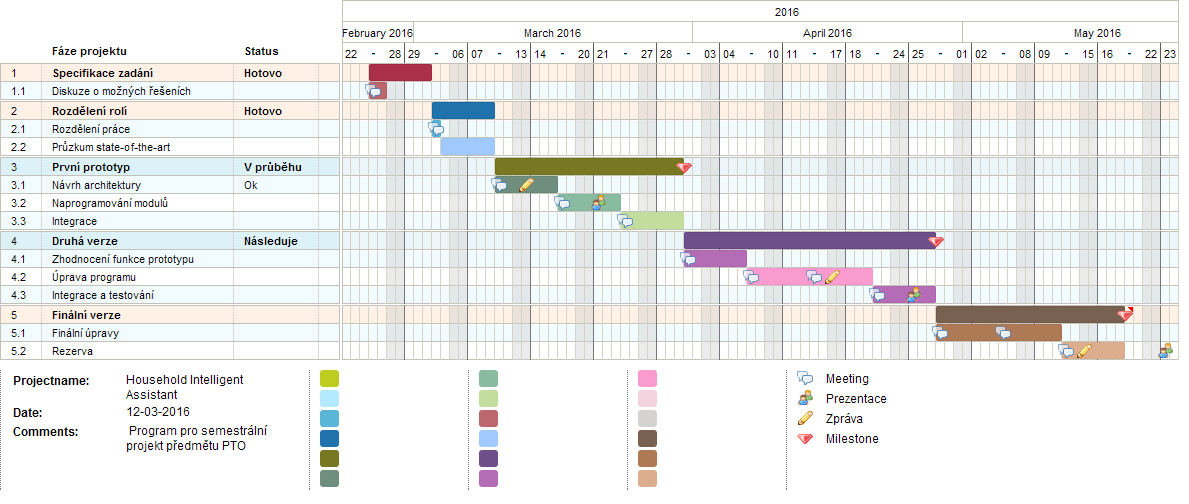
\includegraphics[height = 0.6\textheight ]{PTO-Gantt.png}
	\caption{Harmonogram projektu graficky znázorněn formou Ganttova diagramu s klíčovými milníky.}
	\label{fig:diagram gantt}
	\end{center}
\end{figure}
\vfill
\end{landscape}

\end{document}
